\section{实验与讨论}\label{sec:exp}
本节考察三个问题：按问题类型选择证据能否优于固定传输同一种表示；
逐样本预测如何改变准确率与能耗的取舍；更换接收器后，路由器是否仍然有效。
这些问题分别评估，不预设某一种策略在所有设置中均最优。

\subsection{实验设置}\label{subsec:setup}
\paragraph{数据集与划分}
VisDrone-DET~\cite{zhu2021visdrone} 提供 $548$ 张航拍图像，
DroneVehicle~\cite{sun2022dronevehicle} 提供 $490$ 张图像。
问题包括存在性、计数、数量比较、共现和阈值判断。
对图像标识计算 $\mathrm{crc32}\bmod100$：小于 $20$ 为测试集，
不小于 $80$ 为验证集，其余为训练集。
同一图像的全部问题与信噪比回放保持在同一划分。
VisDrone 的训练/验证/测试图像数为 $343/101/104$；
DroneVehicle 为 $275/93/122$。
两个测试集分别包含 $936$ 和 $710$ 个问题。
六个信噪比点产生每种 VisDrone 信道 $5616$ 条决策和 DroneVehicle 的 $4260$ 条决策。
重复日志按图像、问题、信噪比和证据分支去重。

VisDrone 的信道扫描比较固定图像、固定检测证据、类型规则和训练集查表策略。
逐样本比较使用已核验的 AWGN 记录、DroneVehicle 目标数据拟合，
以及后文的匹配接收器实验。
这些是不同的评估设置，不可把汇总值作为同一测试集的结果直接排序。
DroneVehicle 目标数据拟合并不等于 VisDrone 至 DroneVehicle 的零样本迁移。

\paragraph{答案与计数校准}
YOLOv8n 在官方 VisDrone 训练集上训练，与评估图像分离；不在 DroneVehicle 上重新训练。
默认图像接收器为冻结的 Qwen2-VL-2B~\cite{wang2024qwen2vl}，采用贪心解码，最多生成 $24$ 个 token。
检测证据分支对完整接收数据包执行符号操作。
是非题经规范化后精确匹配；计数正确条件为误差不超过
$\max(1,\operatorname{round}(0.1N))$，其中 $N$ 为真实数量。

计数校准仅使用训练图像，按目标类别和信噪比拟合。
真实数量总和与接收数量总和之比截断至 $[0.5,4]$ 后，
仅在不降低训练计数准确率时保留；小于三的计数不变。
参数冻结后用于验证和测试。补充材料保留不校准对照。
校准改变接收端的计数回答，而不是发送端特征。
学习型路由采用原始检测框中核验的传输前数量。

\paragraph{信道与能耗}\label{subsec:energy-exp}
VisDrone 使用 AWGN、Rayleigh 和 Rician，
信噪比为 $\{-5,0,5,10,15,20\}$ dB；
DroneVehicle 使用相同信噪比点的 Rician，$K=6$ dB。
带宽、参考窗口和发射功率分别为 $1$ MHz、$0.3$ s 和 $0.5$ W。
JPEG 编码先降低质量，必要时降低分辨率。
使用原始图像、编码器和随机种子恢复发送载荷，
要求重建后保存的 JPEG 与既有接收图像逐字节相同，才配对原答案与新载荷成本。
VisDrone 的 $9864$ 个、DroneVehicle 的 $2940$ 个图像/信噪比记录全部通过检查；
后者同时核验了 $7320$ 个记录的接收文件路径。
中断按完整 $0.3$ s 窗口计费。检测数据包沿用第~\paperref{subsec:phy}~节的紧凑空口时间模型。

VLM 的每题增量能耗采用 RTX 4060 代理设备在 $5$ dB 工作负载上测得的 $32.31$ J，
在两数据集与各信道条件间固定使用，不代表 DroneVehicle 新测量。
测量在 $20$ s 预热后进行，采样频率约 $8$ Hz。
机载检测采用 $0.4275$ J 的 Jetson 级功率/时延建模值~\cite{nvidia2024orinnano}，不是嵌入式设备实测值。
参考功放效率 $\eta=1$。
\begin{table}[ht]\centering
\caption{能耗核算使用的 GPU 测量。桌面检测器交叉检查不替代机载建模值；VLM 增量能耗为参考边缘开销。}\label{tab:power}
\begin{tabular}{lrrrr}\toprule
阶段 & 功率/W & 时间/(s/项) & 增量能耗/J & 总能耗/J\\\midrule
空闲 & 52.3 & --- & --- & ---\\
YOLOv8n & 58.7 & 0.0104 & 0.066 & 0.61\\
Qwen2-VL-2B & 107.9 & 0.581 & 32.31 & 62.72\\
\bottomrule\end{tabular}
\end{table}

学习型路由对每次查询计入检测；类型规则和查表策略仅在检测分支计入该项。
空口时间按实际所选样本计算，不使用分支平均载荷。
源编码、路由计算、符号解码、飞行、感知、排队和射频电路均未计入。
节能指所定义的无人机与边缘端合计能耗，不是无人机续航测量。

\paragraph{基线与重复运行}
类型规则无需训练。查表策略在训练集的每个问题类型/信噪比格中选择准确率较高分支，
平局选择检测。两分支样本数相同时，这与 Wilson 下界~\cite{wilson1927probable} 的排序一致。
线性路由使用相同输入的两个逻辑回归正确性预测器，
固定 $400$ 步、步长 $0.5$、L2 系数 $0.001$。
MLP 隐藏层为 $32/16$，Adam 学习率 $0.001$、批量 $200$、L2 系数 $0.0001$。
验证 BCE 连续 $10$ 轮未改善至少 $10^{-4}$ 时停止，最多 $300$ 轮，并恢复最佳验证模型。
全部 MLP 比较保留种子 $0$--$9$。

MLP 结果报告十种子均值，标准差仅表示训练随机性，不代表跨独立数据集的不确定性。
同一图像上的问题与信噪比回放并非独立观察。
以下比较为描述性分析，不将小幅均值差异称为统计显著。
补充材料给出来源范围与其他已核验对照。

\subsection{类型路由与证据互补性}
图~\ref{fig:f1} 展示 VisDrone 信道扫描。
类型规则在 AWGN、Rayleigh、Rician 上的六信噪比汇总准确率为
$67.47\%$、$66.92\%$、$67.27\%$，
图像分支为 $60.43\%$、$60.15\%$、$60.63\%$。
简单改变回答路径即可带来准确率收益，无需学习型逐样本选择器。
\begin{figure}[ht]\centering
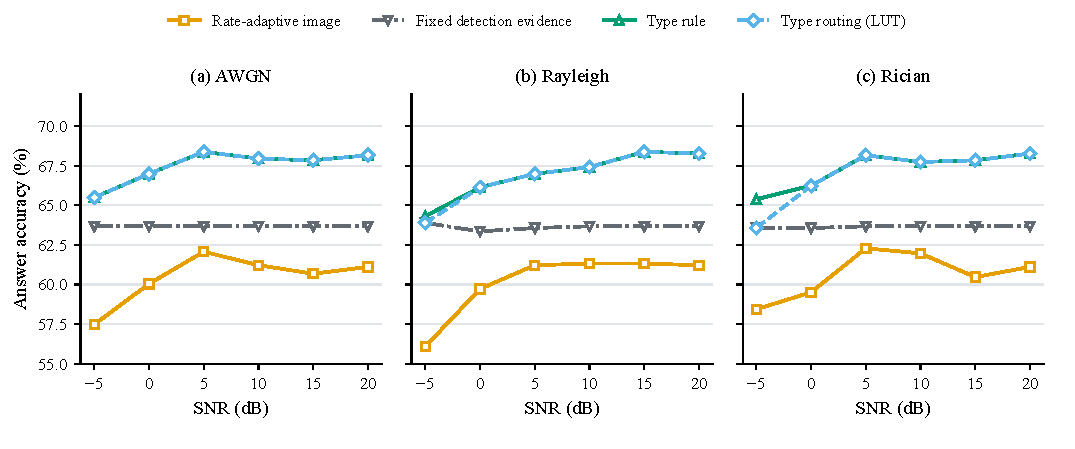
\includegraphics[width=\linewidth]{figures/evidence_final/type_routing.pdf}
\caption{VisDrone 的固定策略比较。每信噪比点 $936$ 个问题，覆盖五类任务。
固定策略没有训练种子误差带。查表策略仅由训练图像拟合。}\label{fig:f1}
\end{figure}
\begin{table}[ht]\centering
\caption{VisDrone 六信噪比汇总准确率（\%）。每种信道包含 $5616$ 条决策。}\label{tab:persample}
\begin{tabular}{lrrr}\toprule
策略 & AWGN & Rayleigh & Rician\\\midrule
图像 & 60.43 & 60.15 & 60.63\\
检测证据 & 63.68 & 63.64 & 63.64\\
类型规则 & 67.47 & 66.92 & 67.27\\
训练集查表 & 67.47 & 66.84 & 66.97\\
\bottomrule\end{tabular}
\end{table}

类型规则每题约 $14.46$ J，图像约 $32.45$ J，系统节能约 $55.4\%$。
规则将 $43.8\%$ 的查询交给图像接收器。
查表策略的汇总准确率相近，但在衰落信道上更少选择图像；
准确率相近既不意味着能耗相同，也不能据此建立统计等效性。

在 Rician VisDrone 上，检测证据对计数、比较、共现分别比图像高
$18.07$、$13.62$、$10.42$ 个百分点；
存在性则是图像高 $8.29$ 个百分点。
阈值问题不满足符号分支总是更好的排序：检测低 $1.44$ 个百分点。
DroneVehicle 上四种计数相关任务均是检测更好，但存在性图像优势仅为 $1.39$ 个百分点。
因此，证据优劣依赖任务和数据集。实验支持设计动机，
却不能证明命题~\paperref{prop:pareto} 的假设在所有设置中成立。
\begin{figure}[ht]\centering
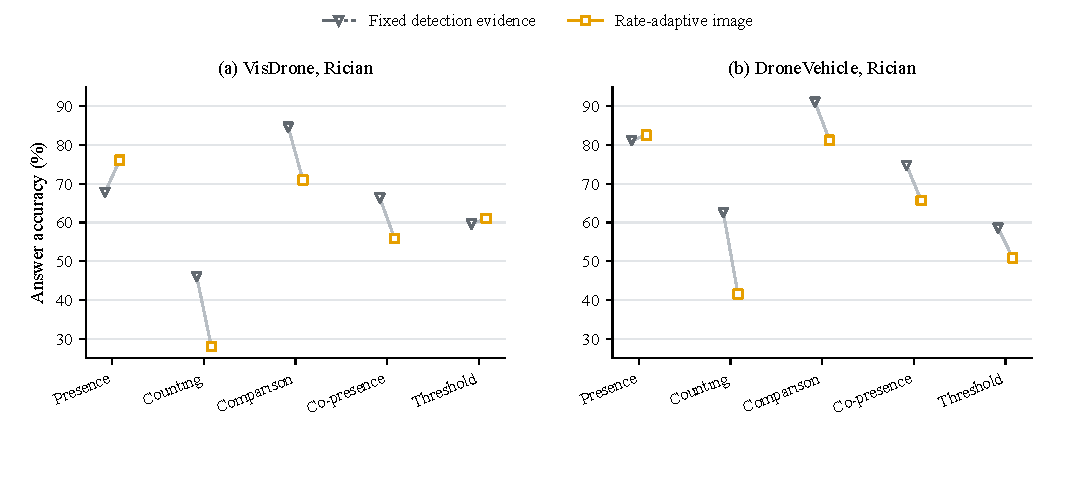
\includegraphics[width=\linewidth]{figures/evidence_final/evidence_complementarity.pdf}
\caption{六个 Rician 信噪比汇总后的分类型准确率。比较在各数据集内部进行，
不代表两个数据集图像或问题逐一匹配。}\label{fig:comp}
\end{figure}

\subsection{逐样本路由与能耗控制}\label{subsec:energyctl}
学习型预测可以利用同一问题类型内的样本差异，但需与简单基线比较。
在已核验的 VisDrone AWGN 上，默认 MLP 为
$67.92\%\pm0.19\%$、每题 $13.38$ J；
线性路由为 $68.02\%$、$11.86$ J；
类型规则为 $67.47\%$、$14.46$ J。
MLP 并未在两个指标上同时优于线性参考。
补充材料中的 AWGN 消融也仅表现出较小的默认准确率变化。
更多输入和非线性结构本身不是工作点更优的证据。

DroneVehicle 评估在目标数据集重新拟合路由器。
默认 MLP 比规则高 $2.97$ 个百分点，却使用 $12.60$ J 而非 $11.21$ J。
全检测仅需 $0.434$ J，达到 $72.46\%$；查表策略在测试集全部选择检测。
线性路由也接近这一低成本端点。
没有明确的准确率要求或能耗代价，就不存在唯一更优策略。
\begin{table}[ht]\centering
\caption{DroneVehicle 目标数据拟合：$122$ 张测试图像、$4260$ 条问题/信噪比决策。MLP 为十种子均值 $\pm$ 样本标准差。}\label{tab:dv}
\begin{tabular}{lrr}\toprule
策略 & 准确率/\% & 能耗/(J/题)\\\midrule
图像 & 64.08 & 32.442\\
检测证据 & 72.46 & 0.434\\
类型规则 & 72.93 & 11.209\\
训练集查表 & 72.46 & 0.434\\
线性，默认 & 72.70 & 2.810\\
线性，验证选价 & 72.46 & 0.434\\
MLP，默认 & $75.91\pm0.21$ & $12.599\pm1.540$\\
MLP，验证选价 & $74.60\pm0.45$ & $4.473\pm1.406$\\
\bottomrule\end{tabular}
\end{table}

候选价格固定为零以及 $10^{-5}$ 至 $10^{-1}$ J$^{-1}$ 间的 $25$ 个对数网格点。
每个种子在验证准确率不低于自身零价格准确率减一个百分点的候选中，
选择验证能耗最低者，平局取较小价格。线性路由采用相同流程。
这是每个预测器自身的相对约束，不是共同绝对准确率目标，也不使用测试答案选价。

图~\ref{fig:f5} 给出全部扫描点与验证选定工作点。
MLP 选价后以 $4.47$ J 达到 $74.60\%$，
比类型规则高 $1.67$ 个百分点、系统能耗低约 $60.1\%$；
相对固定图像节能约 $86.2\%$。
这支持依据计算成本调整证据选择，但不表明 MLP 优于更便宜的全检测，
也不证明该点全局最优。
选价后测试准确率平均下降 $1.31$ 个百分点，超过验证阶段的一点允许量；
验证约束不是测试保证。
\begin{figure}[ht]\centering
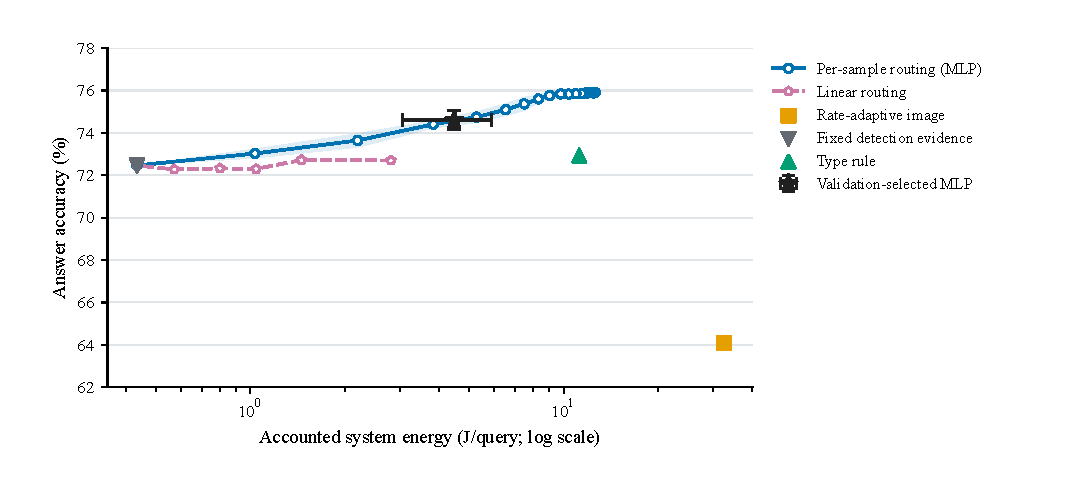
\includegraphics[width=\linewidth]{figures/evidence_final/dv_tradeoff.pdf}
\caption{DroneVehicle 的 $26$ 点价格扫描。MLP 曲线为同一价格下十种子均值，
阴影为准确率的一个样本标准差。星号为各种子验证选点的均值，
双向误差线为两个坐标各自的一个样本标准差；它不一定落在固定价格均值曲线上。
横轴能耗使用对数尺度。}\label{fig:f5}
\end{figure}

\paragraph{系统能耗与无人机能耗}
避免边缘 VLM 推理解释了大部分系统节能。
选价 MLP 每题 $4.47$ J 中，无人机约 $0.45$ J，边缘推理约 $4.02$ J。
固定图像的无人机成本只有 $0.13$ J，而边缘为 $32.31$ J。
类型规则的无人机成本为 $0.33$ J。
因此，在参考配置下，两种路由均降低系统能耗，却增加了相对固定图像的机载建模能耗。
本文收益是通信与推理的联合效率，不是已经证明的飞行时间延长。
\begin{figure}[ht]\centering
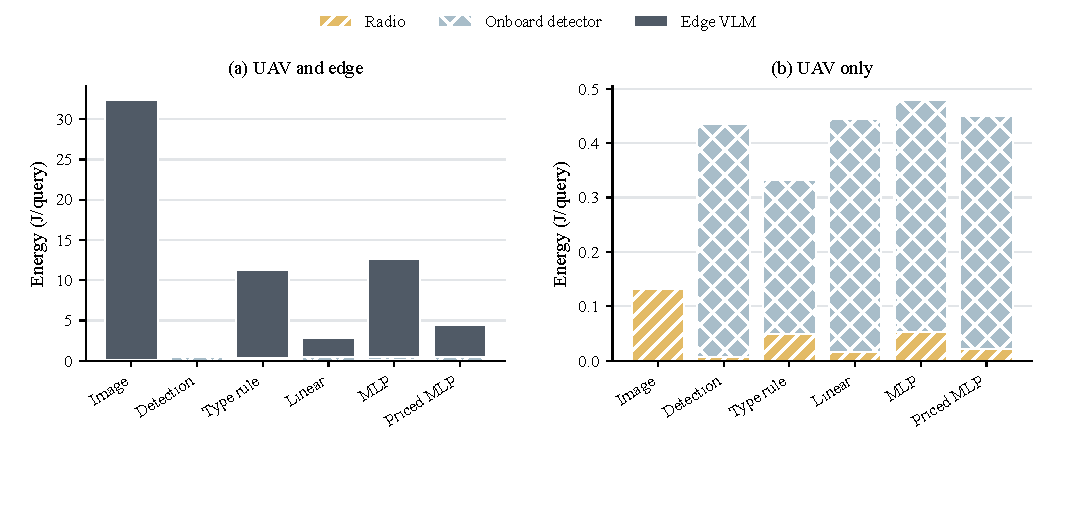
\includegraphics[width=\linewidth]{figures/evidence_final/dv_energy_components.pdf}
\caption{DroneVehicle 能耗分解。右图不包含边缘推理。
MLP 柱为十种子平均分量；机载检测和无线能耗采用模型，边缘推理采用固定测量代理；未计入项见实验设置。}\label{fig:estack}
\end{figure}

\subsection{接收器适配}\label{subsec:crossvlm}
三个接收器 Qwen2-VL-2B、Qwen2.5-VL-3B 和 SmolVLM
使用完全相同的成对问题/信噪比键以及逐字节相同的接收图像。
共享检测记录和仅公共训练集拟合的计数校准也相同。
公共训练/验证/测试决策数为 $9150/2646/2808$。
每个接收器分别拟合线性路由和十种子 MLP，设置相同。
另将在该公共训练集上拟合的 Qwen2 路由器冻结，
把不变的选择直接交给另外两个接收器，评价其目标答案。
\begin{table}[ht]\centering
\caption{匹配接收器准确率（\%），$\lambda=0$。MLP 为十种子均值 $\pm$ 样本标准差；冻结源路由器未经目标接收器拟合。}\label{tab:crossvlm}
\small
\begin{tabular}{lrrr}\toprule
策略 & Qwen2 & Qwen2.5 & SmolVLM\\\midrule
图像 & 62.93 & 62.57 & 59.29\\
检测证据 & 67.09 & 67.09 & 67.09\\
类型规则 & 69.34 & 67.31 & 67.38\\
专用线性路由 & 69.59 & 68.38 & 68.13\\
专用 MLP & $69.63\pm0.38$ & $68.62\pm0.28$ & $69.29\pm0.57$\\
冻结源 MLP & --- & $68.28\pm0.43$ & $67.09\pm0.90$\\
\bottomrule\end{tabular}
\end{table}

MLP 相对线性的均值优势为 $0.04$、$0.25$、$1.16$ 个百分点，
说明专用拟合对不同接收器的价值不同。
冻结 Qwen2 路由后，SmolVLM 比专用拟合低 $2.20$ 个百分点。
这支持按回答机制进行适配，不支持任意接收器独立的路由保证。
公共测试覆盖 $104$ 张图像，但存在性和计数仅来自其中 $26$ 张，其他三类覆盖全部图像。
不能将此汇总准确率与原完整 VisDrone 工作负载直接比较。
五类均齐全的图像子集在补充材料单列。
由于没有替代接收器的独立能耗测量，本组报告准确率与分支使用率，不报告节能率。

\subsection{讨论与局限}\label{sec:limits}
证据选择联合决定通信内容与回答计算。
简单类型规则已捕捉到部分问题间差异；
逐样本预测提供其他工作点，但收益依赖数据集、接收器和图像推理成本。
相对线性参考的小幅改善不足以支持非线性路由普遍更优。

评估仅覆盖有限航拍图像上的结构化生成问题。
问题与信噪比回放共享图像，图像互斥也不能证明邻近场景相互独立。
DroneVehicle 只有 Rician，并在目标训练集拟合路由；
匹配接收器的不同问题类型覆盖不均。
这些实验不证明开放语言能力或对另一航拍数据集的零样本泛化。

能耗结合边缘设备测量与机载、无线成本模型，
假定每个问题独立、无批处理，也不在同图问题间分摊检测。
检测空口时间与参考窗口中断模型并非已验证的有限码长链路。
源编码、射频电路与若干计算成本仍未计入。
嵌入式设备测量和在线评估仍是确认真实时延及无人机电池效应所需的工作。
